\documentclass[12pt,english,nohyper]{tufte-handout}\usepackage[]{graphicx}\usepackage[]{color}
%% maxwidth is the original width if it is less than linewidth
%% otherwise use linewidth (to make sure the graphics do not exceed the margin)
\makeatletter
\def\maxwidth{ %
  \ifdim\Gin@nat@width>\linewidth
    \linewidth
  \else
    \Gin@nat@width
  \fi
}
\makeatother

\definecolor{fgcolor}{rgb}{0.345, 0.345, 0.345}
\newcommand{\hlnum}[1]{\textcolor[rgb]{0.686,0.059,0.569}{#1}}%
\newcommand{\hlstr}[1]{\textcolor[rgb]{0.192,0.494,0.8}{#1}}%
\newcommand{\hlcom}[1]{\textcolor[rgb]{0.678,0.584,0.686}{\textit{#1}}}%
\newcommand{\hlopt}[1]{\textcolor[rgb]{0,0,0}{#1}}%
\newcommand{\hlstd}[1]{\textcolor[rgb]{0.345,0.345,0.345}{#1}}%
\newcommand{\hlkwa}[1]{\textcolor[rgb]{0.161,0.373,0.58}{\textbf{#1}}}%
\newcommand{\hlkwb}[1]{\textcolor[rgb]{0.69,0.353,0.396}{#1}}%
\newcommand{\hlkwc}[1]{\textcolor[rgb]{0.333,0.667,0.333}{#1}}%
\newcommand{\hlkwd}[1]{\textcolor[rgb]{0.737,0.353,0.396}{\textbf{#1}}}%

\usepackage{framed}
\makeatletter
\newenvironment{kframe}{%
 \def\at@end@of@kframe{}%
 \ifinner\ifhmode%
  \def\at@end@of@kframe{\end{minipage}}%
  \begin{minipage}{\columnwidth}%
 \fi\fi%
 \def\FrameCommand##1{\hskip\@totalleftmargin \hskip-\fboxsep
 \colorbox{shadecolor}{##1}\hskip-\fboxsep
     % There is no \\@totalrightmargin, so:
     \hskip-\linewidth \hskip-\@totalleftmargin \hskip\columnwidth}%
 \MakeFramed {\advance\hsize-\width
   \@totalleftmargin\z@ \linewidth\hsize
   \@setminipage}}%
 {\par\unskip\endMakeFramed%
 \at@end@of@kframe}
\makeatother

\definecolor{shadecolor}{rgb}{.97, .97, .97}
\definecolor{messagecolor}{rgb}{0, 0, 0}
\definecolor{warningcolor}{rgb}{1, 0, 1}
\definecolor{errorcolor}{rgb}{1, 0, 0}
\newenvironment{knitrout}{}{} % an empty environment to be redefined in TeX

\usepackage{alltt}
\usepackage[T1]{fontenc}
\usepackage[utf8]{inputenc}
\usepackage{longtable}
\usepackage{wrapfig}
\usepackage{hyperref}
\usepackage{graphicx}
\usepackage[space]{grffile}
\usepackage{geometry}
\usepackage{pgffor}
%\usepackage{caption}
\usepackage{calc}
\usepackage{enumitem}
\usepackage{microtype}
%\usepackage{floatrow} % test for caption below
\usepackage{tabularx}
%\usepackage[capposition=bottom]{floatrow}
\IfFileExists{upquote.sty}{\usepackage{upquote}}{}
\begin{document}



\centerline{\Large\bf Statistics 101 Homework Short Report for Topic 06 AB}
\vspace{1cm}

\begin{marginfigure}
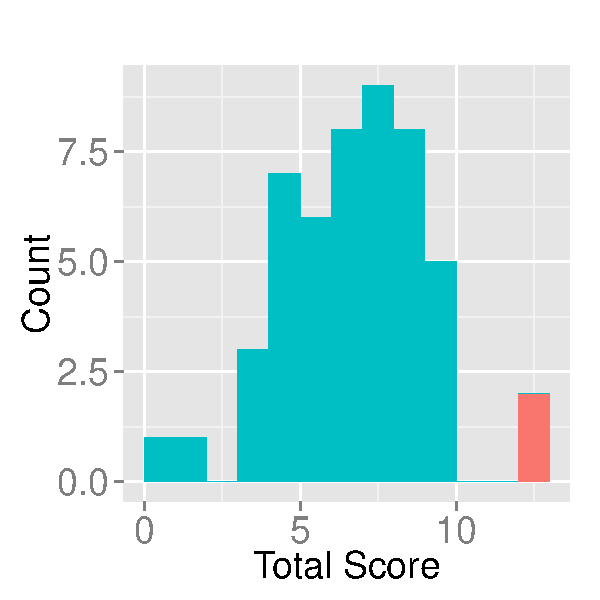
\includegraphics[width=0.98\linewidth]{Topic06_AB_score}
\caption{\label{mar:hist}Histogram of scores. Blue data represent scores less than 80 percent.}
\end{marginfigure}

% latex table generated in R 3.2.2 by xtable 1.7-4 package
% Thu Sep 17 11:42:41 2015
\begin{longtable}{llllllll}
  \hline
Mean & Std.dev &   & Min & Q1 & Median & Q3 & Max \\ 
  \hline
6.24 & 2.38 &  & 0.00 & 5.00 & 6.00 & 8.00 & 12.00 \\ 
  (25\%) & (9.5\%) &  & (0\%) & (20\%) & (24\%) & (32\%) & (48\%) \\ 
   \hline
\hline
\caption{Summary statistics of the scores} 
\label{tab:summary}
\end{longtable}




\newif\ifPositive

\Positivetrue

\ifPositive
Each of the 50 students were given 25 questions from a bank of 89 questions. Figure \ref{mar:hist} and Table \ref{tab:summary} give the overall summary of student performance. Table \ref{tab:studentsbelow80} lists the 50 students who did not perform well on this homework. Table \ref{tab:QuestionSet_summary} and Figure \ref{fig:LearningObj_summary} provide summary statistics of the scores per question set and learning outcome.
\else
Each of the 50 students were given 25 questions from a bank of 89 questions. Figure \ref{mar:hist} and Table \ref{tab:summary} give the overall summary of student performance. Table \ref{tab:QuestionSet_summary} and Figure \ref{fig:LearningObj_summary} provide summary statistics of the scores per question set and learning outcome.
\fi

\bigskip{}

\begin{fullwidth}
\makeatletter\setlength\hsize{\@tufte@fullwidth}\makeatother
% latex table generated in R 3.2.2 by xtable 1.7-4 package
% Thu Sep 17 11:42:41 2015
\begin{longtable}{rr|lr|lr|lr}
  \hline
  & \% Correct &   & \% Correct &   & \% Correct &   & \% Correct \\ 
  \hline
w.introstat40 & 48.00 & w.introStat59 & 32.00 & w.introstat43 & 24.00 & w.introstat23 & 16.00 \\ 
  w.introStat50 & 48.00 & w.introstat69 & 32.00 & w.introStat51 & 24.00 & w.introstat29 & 16.00 \\ 
  w.introstat26 & 36.00 & w.introstat31 & 28.00 & w.introStat53 & 24.00 & w.introstat36 & 16.00 \\ 
  w.introstat39 & 36.00 & w.introstat35 & 28.00 & w.introstat66 & 24.00 & w.introstat46 & 16.00 \\ 
  w.introstat42 & 36.00 & w.introstat44 & 28.00 & w.introstat67 & 24.00 & w.introStat56 & 16.00 \\ 
  w.introStat52 & 36.00 & w.introstat48 & 28.00 & w.introstat70 & 24.00 & w.introstat68 & 16.00 \\ 
  w.introstat65 & 36.00 & w.introStat54 & 28.00 & w.introstat21 & 20.00 & w.introstat24 & 12.00 \\ 
  w.introstat33 & 32.00 & w.introStat58 & 28.00 & w.introstat28 & 20.00 & w.introstat27 & 12.00 \\ 
  w.introstat34 & 32.00 & w.introstat61 & 28.00 & w.introstat38 & 20.00 & w.introstat30 & 12.00 \\ 
  w.introstat37 & 32.00 & w.introstat62 & 28.00 & w.introstat47 & 20.00 & w.introstat64 & 4.00 \\ 
  w.introstat45 & 32.00 & w.introstat63 & 28.00 & w.introStat57 & 20.00 & w.introstat25 & 0.00 \\ 
  w.introstat49 & 32.00 & w.introstat32 & 24.00 & w.introstat60 & 20.00 &  &  \\ 
  w.introStat55 & 32.00 & w.introstat41 & 24.00 & w.introstat22 & 16.00 &  &  \\ 
   \hline
\hline
\caption{The  50 students whose percentages are less than 80\%.} 
\label{tab:studentsbelow80}
\end{longtable}

\end{fullwidth}



\vspace{-2mm}

\noindent
\underline{Topic 06 Learning Outcomes:}
\vspace{2mm}

\begin{fullwidth}
\begin{enumerate}[label=\Alph*.,itemsep=-\parsep,leftmargin=*]
  \item
Use standardizing to determine how many standard deviations an observation is away from the mean value.
\item Use z-scores to compare observations for different quantitative variables.
\item Explain how standardizing affects the shape, center, and variability of the distribution of a quantitative variable.
\item Determine which quantitative variables could be modeled using the normal distribution by interpreting graphical representations of the variable.
\item Apply the 68-95-99.
\item Find percentile or area values for any given observation from a normal distribution.
\item Find the value of an observation when given a percentile or area value from the normal distribution.

\end{enumerate}
\end{fullwidth}



\vspace{5mm}

%\begin{fullwidth} %ADDED NOW
%\makeatletter\setlength\hsize{\@tufte@fullwidth}\makeatother %ADDED NOW
%\begin{centering}
\begin{figure}[!ht]
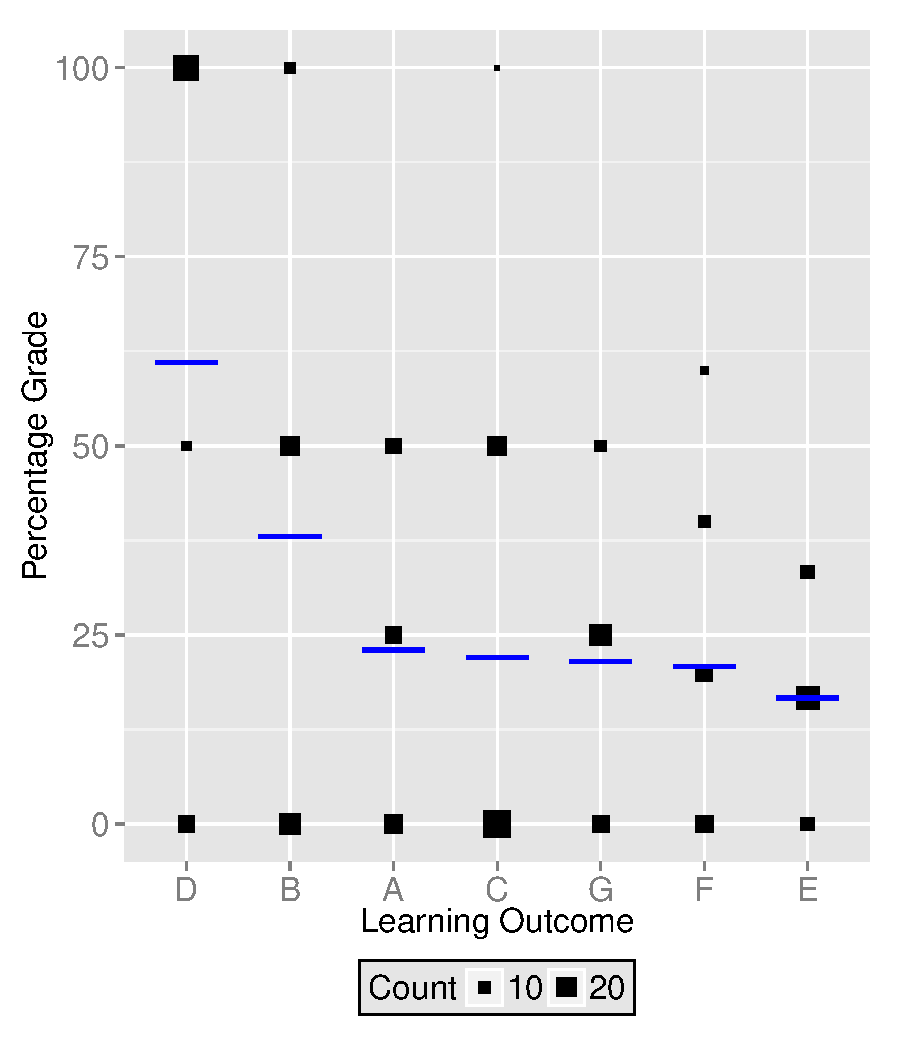
\includegraphics[width=\linewidth]{Topic06_AB_LearningObj_boxplot.pdf}
\caption{Fluctuation diagram of percentage correct by learning outcome. Mean scores are drawn as blue bars.}
\label{fig:LearningObj_summary}
\end{figure}
%\end{centering}
%\end{fullwidth} %ADDED NOW

\begin{fullwidth}
\makeatletter\setlength\hsize{\@tufte@fullwidth}\makeatother
% latex table generated in R 3.2.2 by xtable 1.7-4 package
% Thu Sep 17 11:42:42 2015
\begin{longtable}{cc|ccc|ccc}
  \hline
LO & Qset & \# & Mean & Std.dev & Min & Median & Max \\ 
  \hline
D & I &   2 & \color{red}{64} & 48.49 & 0.00 & 100.00 & 100.00 \\ 
  D & J &   4 & \color{red}{58} & 49.86 & 0.00 & 100.00 & 100.00 \\ 
  A & B &   4 & \color{red}{48} & 50.47 & 0.00 & 0.00 & 100.00 \\ 
  A & A &   4 & \color{red}{44} & 50.14 & 0.00 & 0.00 & 100.00 \\ 
  B & E &   1 & \color{red}{40} & 49.49 & 0.00 & 0.00 & 100.00 \\ 
  B & F &   1 & \color{red}{36} & 48.49 & 0.00 & 0.00 & 100.00 \\ 
  F & M &   5 & \color{red}{36} & 48.49 & 0.00 & 0.00 & 100.00 \\ 
  F & Q &   5 & \color{red}{30} & 46.29 & 0.00 & 0.00 & 100.00 \\ 
  G & S &   5 & \color{red}{26} & 44.31 & 0.00 & 0.00 & 100.00 \\ 
  G & U &   5 & \color{red}{26} & 44.31 & 0.00 & 0.00 & 100.00 \\ 
  C & H &   1 & \color{red}{24} & 43.14 & 0.00 & 0.00 & 100.00 \\ 
  E & L &   9 & \color{red}{23.33} & 25.42 & 0.00 & 33.33 & 66.67 \\ 
  C & G &   1 & \color{red}{20} & 40.41 & 0.00 & 0.00 & 100.00 \\ 
  F & N &   5 & \color{red}{18} & 38.81 & 0.00 & 0.00 & 100.00 \\ 
  G & R &   5 & \color{red}{18} & 38.81 & 0.00 & 0.00 & 100.00 \\ 
  G & T &   5 & \color{red}{16} & 37.03 & 0.00 & 0.00 & 100.00 \\ 
  F & O &   5 & \color{red}{14} & 35.05 & 0.00 & 0.00 & 100.00 \\ 
  E & K &   9 & \color{red}{10} & 15.43 & 0.00 & 0.00 & 33.33 \\ 
  F & P &   5 & \color{red}{6} & 23.99 & 0.00 & 0.00 & 100.00 \\ 
  A & C &   4 & \color{red}{0} & 0.00 & 0.00 & 0.00 & 0.00 \\ 
  A & D &   4 & \color{red}{0} & 0.00 & 0.00 & 0.00 & 0.00 \\ 
   \hline
\hline
\caption{Summary statistics of the question sets. Rows are sorted by mean scores, which are marked red if less than 80 percent.} 
\label{tab:QuestionSet_summary}
\end{longtable}

\end{fullwidth}

\end{document}
